\section{GRU Activations} % (fold)
\label{sec:gru_activations}
\begin{figure*}[h!]
    \centering
    \setkeys{Gin}{height=.28\textheight}
	\hspace*{\fill}
    \subbottom[\label{fig:activations:26}]{
        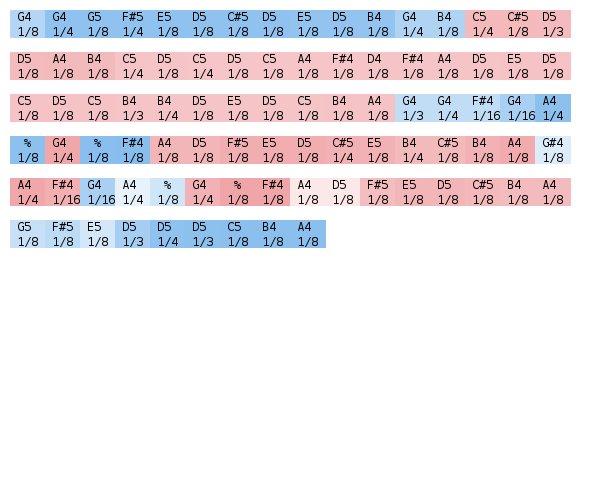
\includegraphics{model_1_with_50p_dropout_gru_100_bs_10_e_200_Fiddle Hill Jig_gruActivations_gru26}
    }
    \hfill
    \subbottom[\label{fig:activations:50}]{
        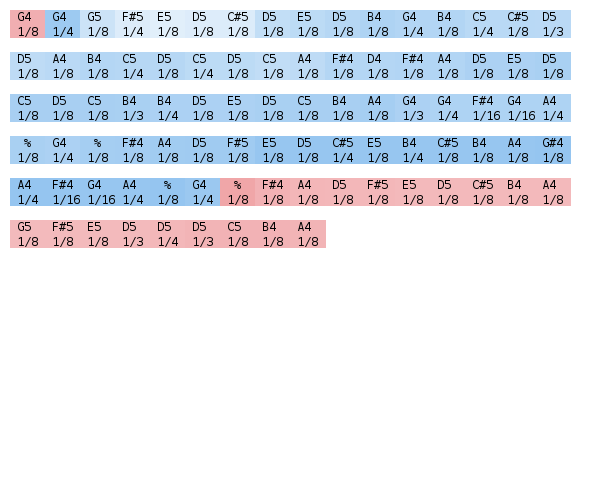
\includegraphics{model_1_with_50p_dropout_gru_100_bs_10_e_200_Fiddle Hill Jig_gruActivations_gru50}
    }
	\hspace*{\fill}
    \caption{GRU Activations, $h\idx{k}\order{t}$, for \subcaptionref{fig:activations:26} unit $k=26$, which shows a higher response to the combination of the pitch G and F\#, and \subcaptionref{fig:activations:50} unit $k=50$, which shows a higher response in the beginning and end of the melody.)
    }
    \label{fig:activations}
\end{figure*}

% section gru_activations (end)

\section{GRU Weights} % (fold)
\label{sec:gru_weights}
\begin{figure*}[h!]
    \centering
    \setkeys{Gin}{height=.23\textheight}
	\hspace*{\fill}
    \subbottom[\label{fig:model_1:weights_pos:horz}]{
        \includegraphics{model_1_with_50p_dropout_gru_100_bs_10_e_200_horzWeights_mean}
    }
    \hfill
    \subbottom[\label{fig:model_1:weights_pos:vert}]{
        \includegraphics{model_1_with_50p_dropout_gru_100_bs_10_e_200_vertWeights_mean}
    }
	\hspace*{\fill}
    \caption{Mean over the three kinds of GRU weights (Update, Reset and Candidate), for \subcaptionref{fig:model_1:weights_pos:horz} horizontal weights $\mat{W}\idx{h}$ and \subcaptionref{fig:model_1:weights_pos:vert} vertical weights $\mat{W}\idx{x}$ recorded after each epoch.
 	}
    \label{fig:model_1:weights_pos}
\end{figure*}

\begin{figure*}[h!]
    \centering
    \setkeys{Gin}{height=.23\textheight}
	\hspace*{\fill}
    \subbottom[\label{fig:model_1:weights_pos:horz}]{
        \includegraphics{model_1_with_50p_dropout_gru_100_bs_10_e_200_horzWeights_norm}
    }
    \hfill
    \subbottom[\label{fig:model_1:weights_pos:vert}]{
        \includegraphics{model_1_with_50p_dropout_gru_100_bs_10_e_200_vertWeights_norm}
    }
	\hspace*{\fill}
    \caption{Frobenius norm over the three kinds of GRU weights (Update, Reset and Candidate), for \subcaptionref{fig:model_1:weights_pos:horz} horizontal weights $\mat{W}\idx{h}$ and \subcaptionref{fig:model_1:weights_pos:vert} vertical weights $\mat{W}\idx{x}$ recorded after each epoch.
 	}
    \label{fig:model_1:weights_pos}
\end{figure*}

\begin{figure*}[h!]
    \centering
    \setkeys{Gin}{height=.23\textheight}
	\hspace*{\fill}
    \subbottom[\label{fig:model_1:weights_pos:horz}]{
        \includegraphics{model_1_with_50p_dropout_gru_100_bs_10_e_200_horzWeights_pos}
    }
    \hfill
    \subbottom[\label{fig:model_1:weights_pos:vert}]{
        \includegraphics{model_1_with_50p_dropout_gru_100_bs_10_e_200_vertWeights_pos}
    }
	\hspace*{\fill}
    \caption{Fraction of positive values in three kinds of GRU weights (Update, Reset and Candidate), for \subcaptionref{fig:model_1:weights_pos:horz} horizontal weights $\mat{W}\idx{h}$ and \subcaptionref{fig:model_1:weights_pos:vert} vertical weights $\mat{W}\idx{x}$ recorded after each epoch.
 	}
    \label{fig:model_1:weights_pos}
\end{figure*}


\begin{figure*}[h!]
    \centering
    \setkeys{Gin}{height=.23\textheight}
	\hspace*{\fill}
    \subbottom[\label{fig:model_1:weights_pos:horz}]{
        \includegraphics{model_1_with_50p_dropout_gru_100_bs_10_e_200_horzWeights_mean}
    }
    \hfill
    \subbottom[\label{fig:model_1:weights_pos:vert}]{
        \includegraphics{model_1_with_50p_dropout_gru_100_bs_10_e_200_vertWeights_mean}
    }
	\hspace*{\fill}
    \caption{Mean over the three kinds of GRU weights (Update, Reset and Candidate), for \subcaptionref{fig:model_1:weights_pos:horz} horizontal weights $\mat{W}\idx{h}$ and \subcaptionref{fig:model_1:weights_pos:vert} vertical weights $\mat{W}\idx{x}$ recorded after each epoch.
 	}
    \label{fig:model_1:weights_pos}
\end{figure*}

\begin{figure*}[h!]
    \centering
    \setkeys{Gin}{height=.23\textheight}
	\hspace*{\fill}
    \subbottom[\label{fig:model_1:weights_pos:horz}]{
        \includegraphics{model_1_with_50p_dropout_gru_100_bs_10_e_200_horzWeights_norm}
    }
    \hfill
    \subbottom[\label{fig:model_1:weights_pos:vert}]{
        \includegraphics{model_1_with_50p_dropout_gru_100_bs_10_e_200_vertWeights_norm}
    }
	\hspace*{\fill}
    \caption{Frobenius norm over the three kinds of GRU weights (Update, Reset and Candidate), for \subcaptionref{fig:model_1:weights_pos:horz} horizontal weights $\mat{W}\idx{h}$ and \subcaptionref{fig:model_1:weights_pos:vert} vertical weights $\mat{W}\idx{x}$ recorded after each epoch.
 	}
    \label{fig:model_1:weights_pos}
\end{figure*}

\begin{figure*}[h!]
    \centering
    \setkeys{Gin}{height=.23\textheight}
	\hspace*{\fill}
    \subbottom[\label{fig:model_1:weights_pos:horz}]{
        \includegraphics{model_1_with_50p_dropout_gru_100_bs_10_e_200_horzWeights_pos}
    }
    \hfill
    \subbottom[\label{fig:model_1:weights_pos:vert}]{
        \includegraphics{model_1_with_50p_dropout_gru_100_bs_10_e_200_vertWeights_pos}
    }
	\hspace*{\fill}
    \caption{Fraction of positive values in three kinds of GRU weights (Update, Reset and Candidate), for \subcaptionref{fig:model_1:weights_pos:horz} horizontal weights $\mat{W}\idx{h}$ and \subcaptionref{fig:model_1:weights_pos:vert} vertical weights $\mat{W}\idx{x}$ recorded after each epoch.
 	}
    \label{fig:model_1:weights_pos}
\end{figure*}


% section gru_weights (end)

\section{Histogram over note durations} % (fold)
\label{sec:histogram_over_note_durations}
\begin{figure*}
    \centering
    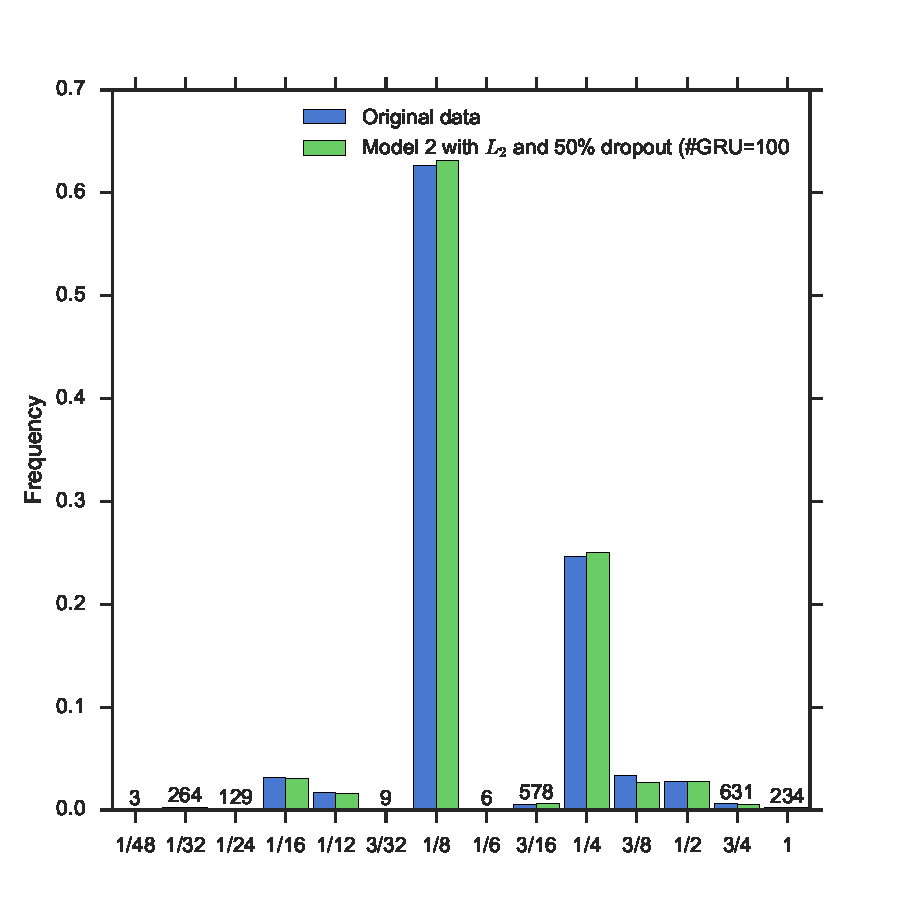
\includegraphics[width=.8\textwidth]{models_duration_freq_barplot}
    \caption{Histograms showing statistical frequency of duration classes in the (blue) original data and in the (green) reconstructions produced by model type 2 with dropout of 50\% and $L_2$-regularization.}
    \label{fig:histogram:duration}
\end{figure*}
% section histogram_over_note_durations (end)